\section{Yau contest}

\begin{figure}[H]
\centering
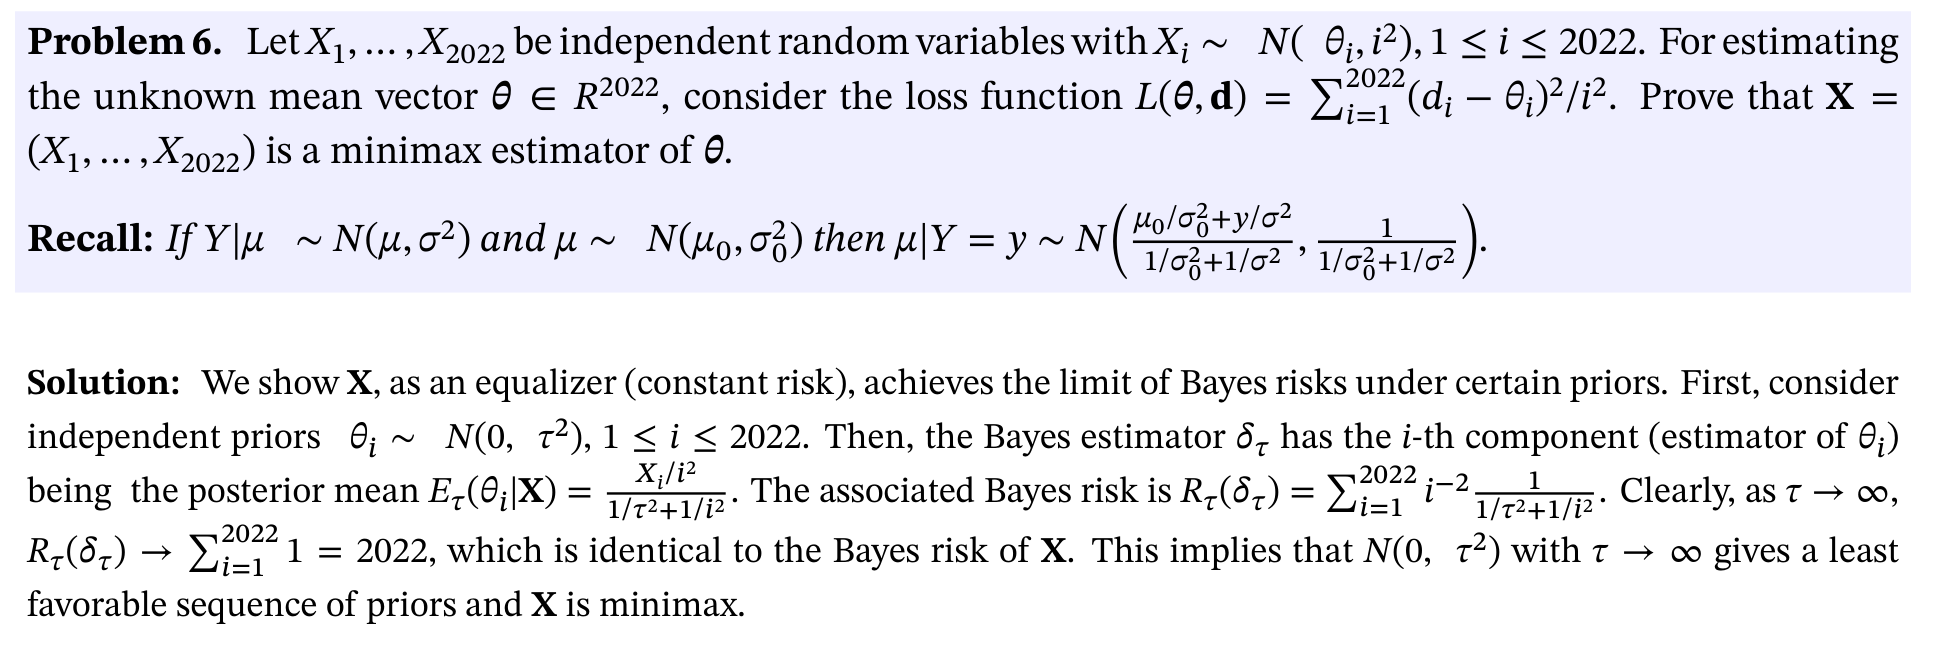
\includegraphics[width=\textwidth]{1-yau-contest-2025051416.png}
% \caption{}
\label{}
\end{figure}

Okay, this problem (Problem 6 from your image) is from the area of statistical decision theory, specifically focusing on estimation theory and minimax estimators. Since you're a beginner in statistics, understanding this problem and its solution will require familiarity with several key concepts.

Here's a breakdown of the topics and materials you'll need to study:

\textbf{I. Foundational Probability and Statistics Concepts:}

\begin{enumerate}
	\item \textbf{Random Variables:}
	\begin{itemize}
		\item \textbf{Definition:} What a random variable is (discrete and continuous).
		\item \textbf{Probability Distributions:} Understanding probability mass functions (PMF) for discrete variables and probability density functions (PDF) for continuous variables.
		\item \textbf{Expected Value (Mean):} $\mathbb{E}[X]$.
		\item \textbf{Variance:} $\text{Var}(X) = \mathbb{E}[(X - \mathbb{E}[X])^2]$.
	\end{itemize}
	\item \textbf{Specific Probability Distributions:}
	\begin{itemize}
		\item \textbf{Normal (Gaussian) Distribution:} $N(\mu, \sigma^2)$.
		\begin{itemize}
			\item Its PDF: $f(x; \mu, \sigma^2) = \frac{1}{\sigma\sqrt{2\pi}} e^{-\frac{(x-\mu)^2}{2\sigma^2}}$.
			\item Properties: Mean $\mu$, variance $\sigma^2$.
			\item The problem states $X_i \sim N(\theta_i, i^2)$. This means each $X_i$ is normally distributed with mean $\theta_i$ and variance $i^2$.
		\end{itemize}
	\end{itemize}
	\item \textbf{Independent Random Variables:}
	\begin{itemize}
		\item Understanding what it means for random variables to be independent. This is crucial as the problem states $X_1, \ldots, X_{2022}$ are independent.
	\end{itemize}
\end{enumerate}

\textbf{II. Statistical Estimation Theory:}

\begin{enumerate}
	\item \textbf{Parameter Estimation:}
	\begin{itemize}
		\item The goal is to estimate an unknown parameter (here, the mean vector $\theta = (\theta_1, \ldots, \theta_{2022})$) based on observed data (here, $X = (X_1, \ldots, X_{2022})$).
		\item \textbf{Estimator:} A function of the data used to estimate the parameter. In this problem, the estimator being considered is $\mathbf{X}$ itself, meaning $d_i = X_i$ is used to estimate $\theta_i$.
	\end{itemize}
	\item \textbf{Loss Function $L(\theta, d)$:}
	\begin{itemize}
		\item A function that quantifies the "cost" or "loss" incurred when the true parameter is $\theta$ and our estimate is $d$.
		\item In this problem, the loss function is a \textbf{weighted squared error loss}:
\[
L(\theta, d) = \sum_{i=1}^{2022} \frac{(d_i - \theta_i)^2}{i^2}
\]This means errors in estimating $\theta_i$ are weighted by $1/i^2$. Errors for components with smaller $i$ (and thus smaller variance $i^2$ for $X_i$) are penalized more heavily relative to their scale if the $i^2$ in the denominator were not there. The $i^2$ in the denominator effectively normalizes the squared error by the variance of the observation $X_i$ if $d_i=X_i$.
	\end{itemize}
	\item \textbf{Risk Function $R(\theta, \delta)$:}
	\begin{itemize}
		\item The expected loss of an estimator $\delta$ when the true parameter is $\theta$.
		\item $R(\theta, \delta) = \mathbb{E}[L(\theta, \delta(X)) | \theta]$. The expectation is taken over the distribution of $X$, given $\theta$.
		\item For the estimator $\delta(X) = X$ (meaning $d_i = X_i$):
\[
R(\theta, X) = \mathbb{E}\left[\sum_{i=1}^{2022} \frac{(X_i - \theta_i)^2}{i^2} \middle| \theta\right]
\]\[
R(\theta, X) = \sum_{i=1}^{2022} \frac{1}{i^2} \mathbb{E}[(X_i - \theta_i)^2 | \theta]
\]Since $X_i \sim N(\theta_i, i^2)$, $\mathbb{E}[(X_i - \theta_i)^2 | \theta]$ is the variance of $X_i$, which is $i^2$.
So, $R(\theta, X) = \sum_{i=1}^{2022} \frac{1}{i^2} \cdot i^2 = \sum_{i=1}^{2022} 1 = 2022$.
This shows that the estimator $X$ has a \textbf{constant risk} (it doesn't depend on the true value of $\theta$). An estimator with constant risk is called an \textbf{equalizer rule}.
	\end{itemize}
\end{enumerate}

\textbf{III. Bayesian Statistics (Used in the Proof Strategy):}

\begin{enumerate}
	\item \textbf{Prior Distribution $\pi(\theta)$:}
	\begin{itemize}
		\item In Bayesian statistics, the unknown parameter $\theta$ is treated as a random variable having a prior distribution, which reflects our beliefs about $\theta$ \textit{before} observing data.
		\item The solution considers independent priors $\theta_i \sim N(0, \tau^2)$. This is a common choice for mathematical convenience.
	\end{itemize}
	\item \textbf{Posterior Distribution $p(\theta|X)$:}
	\begin{itemize}
		\item After observing data $X$, the prior belief is updated to a posterior distribution using Bayes' theorem: $p(\theta|X) \propto L(X|\theta) \pi(\theta)$, where $L(X|\theta)$ is the likelihood of the data given the parameter.
	\end{itemize}
	\item \textbf{Bayes Estimator $\delta_\pi(X)$:}
	\begin{itemize}
		\item An estimator that minimizes the \textbf{Bayes risk} (defined below) for a given prior $\pi$.
		\item For squared error loss \[
(d_i - \theta_i)^2
\], the $i$-th component of the Bayes estimator is the mean of the posterior distribution of $\theta_i$: $\delta_{\pi,i}(X) = \mathbb{E}[\theta_i | X]$.
		\item The problem uses a slightly modified loss. For the loss $\frac{(d_i - \theta_i)^2}{i^2}$, the Bayes estimator for $\theta_i$ will still be $\mathbb{E}[\theta_i | X_i]$ (since the $X_i$ and $\theta_i$ are independent across $i$).
		\item The "Recall" part of the problem gives a formula for the posterior mean when the likelihood is normal and the prior is normal (this is a standard result for \textbf{conjugate priors}):
If $Y | \mu \sim N(\mu, \sigma^2)$ and $\mu \sim N(\mu_0, \sigma_0^2)$, then the posterior distribution of $\mu | Y=y$ is also normal:
\[
\mu | Y=y \sim N\left(\frac{\mu_0/\sigma_0^2 + y/\sigma^2}{1/\sigma_0^2 + 1/\sigma^2}, \frac{1}{1/\sigma_0^2 + 1/\sigma^2}\right)
\]The posterior mean is $\mathbb{E}[\mu|Y=y] = \frac{\mu_0/\sigma_0^2 + y/\sigma^2}{1/\sigma_0^2 + 1/\sigma^2}$.
In the problem's context, for estimating $\theta_i$:
$X_i | \theta_i \sim N(\theta_i, i^2)$ (so $X_i$ is $Y$, $\theta_i$ is $\mu$, variance is $i^2$).
Prior $\theta_i \sim N(0, \tau^2)$ (so $\mu_0=0$, prior variance is $\tau^2$).
The Bayes estimator for $\theta_i$ (posterior mean $\mathbb{E}[\theta_i | X_i]$) is:
\[
\mathbb{E}[\theta_i | X_i] = \frac{0/\tau^2 + X_i/i^2}{1/\tau^2 + 1/i^2} = \frac{X_i/i^2}{1/\tau^2 + 1/i^2} = \frac{X_i \tau^2}{i^2 + \tau^2} = \frac{X_i}{1 + i^2/\tau^2}
\]The solution in the image has $\mathbb{E}_c[\theta_i | X] = \frac{X_i/i^2}{1/\tau^2 + 1/i^2}$. This is slightly different from what I derived for the posterior mean.
Let's re-check the posterior mean given in the problem: $\frac{\mu_0/\sigma_0^2 + y/\sigma^2}{1/\sigma_0^2 + 1/\sigma^2}$.
Here: $y \rightarrow X_i$, $\mu \rightarrow \theta_i$, $\sigma^2 \rightarrow i^2$. And for the prior: $\mu_0 \rightarrow 0$, $\sigma_0^2 \rightarrow \tau^2$.
So, $\mathbb{E}[\theta_i | X_i] = \frac{0/\tau^2 + X_i/i^2}{1/\tau^2 + 1/i^2} = \frac{X_i/i^2}{(i^2+\tau^2)/(i^2\tau^2)} = \frac{X_i \tau^2}{i^2+\tau^2}$.
The solution's notation $\mathbb{E}_c(\theta_i|X) = \frac{X_i/i^2}{1/\tau^2 + 1/i^2}$ is indeed the posterior mean, which simplifies to $\frac{X_i \tau^2}{i^2+\tau^2}$.
	\end{itemize}
	\item \textbf{Bayes Risk $r(\pi, \delta)$ (or $R_c(\delta_\tau)$ in the solution):}
	\begin{itemize}
		\item The expected risk with respect to the prior distribution of $\theta$: $r(\pi, \delta) = \mathbb{E}_\pi[R(\theta, \delta)] = \int R(\theta, \delta) \pi(\theta) d\theta$.
		\item The Bayes estimator $\delta_\pi$ minimizes this Bayes risk. The minimum Bayes risk is $r(\pi) = r(\pi, \delta_\pi)$.
		\item The solution calculates the Bayes risk for the Bayes estimator $\delta_\tau$ (where $\tau$ parameterizes the prior variance).
$R_c(\delta_\tau) = \sum_{i=1}^{2022} \mathbb{E}\left[\frac{(\mathbb{E}[\theta_i|X_i] - \theta_i)^2}{i^2}\right]$. This is not quite right.
The Bayes risk for $\delta_\tau$ is $\mathbb{E}_{\theta, X} \left[ \sum \frac{(\delta_{\tau,i}(X) - \theta_i)^2}{i^2} \right]$.
It's also $\mathbb{E}_\theta [ R(\theta, \delta_\tau) ]$.
Alternatively, for squared error type losses, the Bayes risk of the Bayes estimator $\mathbb{E}[\theta|X]$ is $\mathbb{E}_X[\text{Var}(\theta|X)]$.
The solution states $R_c(\delta_\tau) = \sum_{i=1}^{2022} \frac{1}{i^2} \frac{\tau^{-2}}{1/\tau^2+1/i^2}$.
This term $\frac{\tau^{-2}}{1/\tau^2+1/i^2}$ is $\mathbb{E}[(\delta_{\tau,i}(X_i)-\theta_i)^2]$ or related to posterior variance.
The posterior variance is $\text{Var}(\theta_i|X_i) = \frac{1}{1/\tau^2 + 1/i^2} = \frac{i^2\tau^2}{i^2+\tau^2}$.
The Bayes risk for component $i$ under loss $(\delta_i - \theta_i)^2$ is $\mathbb{E}_X[\text{Var}(\theta_i|X)]$.
So for loss $\frac{(\delta_i - \theta_i)^2}{i^2}$, it would be $\frac{1}{i^2} \mathbb{E}_X[\text{Var}(\theta_i|X_i)] = \frac{1}{i^2} \frac{i^2\tau^2}{i^2+\tau^2} = \frac{\tau^2}{i^2+\tau^2}$.
The solution has $\frac{1}{i^2} \frac{1/\tau^2}{1/\tau^2+1/i^2} = \frac{1}{i^2} \frac{1}{1+i^2/\tau^2} = \frac{1}{i^2+\tau^2}$. This is slightly different.
Let's check: The Bayes risk $r(\pi, \delta_\pi) = \mathbb{E}[\text{Var}(\theta_i|X_i)]$ for component $i$ under squared error loss.
For the weighted loss $\frac{L_0}{i^2}$, the Bayes risk for $\theta_i$ is $\frac{1}{i^2}\mathbb{E}[\text{Var}(\theta_i|X_i)] = \frac{1}{i^2}\frac{i^2 \tau^2}{i^2+\tau^2} = \frac{\tau^2}{i^2+\tau^2}$.
The solution states the associated Bayes risk is $R_c(\delta_\tau) = \sum \frac{1}{i^2} \frac{\tau^{-2}}{1/\tau^2+1/i^2} = \sum \frac{1}{i^2} \frac{1/\tau^2}{(i^2+\tau^2)/(i^2\tau^2)} = \sum \frac{1}{i^2} \frac{i^2}{i^2+\tau^2} = \sum \frac{1}{i^2+\tau^2}$.
This formula for the Bayes risk of a Bayes estimator under normal-normal model with weighted squared error loss is a standard result that you'd find in textbooks on Bayesian decision theory.
	\end{itemize}
\end{enumerate}

\textbf{IV. Minimax Estimation:}

\begin{enumerate}
	\item \textbf{Minimax Estimator $\delta^*$:}
	\begin{itemize}
		\item An estimator $\delta^*$ is minimax if it minimizes the maximum possible risk:
\[
\sup_\theta R(\theta, \delta^*) = \inf_\delta \sup_\theta R(\theta, \delta)
\]		\item Finding minimax estimators can be hard.
	\end{itemize}
	\item \textbf{Proving Minimaxity (Key Theorem Used in the Solution):}
A common way to prove an estimator $\delta_0$ is minimax is to:
	\begin{itemize}
		\item Show that $\delta_0$ is an \textbf{equalizer rule}, meaning its risk $R(\theta, \delta_0)$ is constant (doesn't depend on $\theta$). Let this constant risk be $r_0$.
		\item Find a sequence of prior distributions $\pi_k$ such that the Bayes risk of the Bayes estimator for $\pi_k$, denoted $r(\pi_k, \delta_{\pi_k})$, converges to $r_0$ as $k \to \infty$.
\[
\lim_{k\to\infty} r(\pi_k, \delta_{\pi_k}) = r_0
\]	\end{itemize}
If both conditions hold, then $\delta_0$ is minimax.
(This relies on the fact that $\sup_\theta R(\theta, \delta) \ge r(\pi, \delta)$ and $r(\pi, \delta) \ge r(\pi, \delta_\pi)$).
The theorem states: If $\delta_0$ is an equalizer rule with risk $r_0$, and if there's a sequence of priors $\pi_k$ such that the corresponding Bayes risks $r(\pi_k)$ converge to $r_0$, then $\delta_0$ is minimax.
\end{enumerate}

\textbf{Applying the Theorem to the Problem:}

\begin{enumerate}
	\item The estimator $\mathbf{X}$ (where $d_i = X_i$) has a constant risk $R(\theta, \mathbf{X}) = 2022$. So, $\mathbf{X}$ is an equalizer rule.
	\item The solution considers a sequence of priors $\theta_i \sim N(0, \tau^2)$, so $\pi_\tau$ is the prior.
The Bayes risk for this sequence of priors is $R_c(\delta_\tau) = \sum_{i=1}^{2022} \frac{1}{i^2+\tau^2}$ (as per the solution's formula).
	\item The solution then takes the limit as $\tau \to \infty$ (this corresponds to a sequence of priors that become increasingly "non-informative" or "flat").
\[
\lim_{\tau \to \infty} R_c(\delta_\tau) = \lim_{\tau \to \infty} \sum_{i=1}^{2022} \frac{1}{i^2+\tau^2}
\]As $\tau \to \infty$, each term $\frac{1}{i^2+\tau^2} \to 0$.
So, $\lim_{\tau \to \infty} R_c(\delta_\tau) = \sum_{i=1}^{2022} 0 = 0$.
\textbf{There's a discrepancy here.} The constant risk of $\mathbf{X}$ is $2022$. The limit of Bayes risks is $0$.
For $\mathbf{X}$ to be minimax, the limit of Bayes risks should converge to the constant risk of $\mathbf{X}$, which is $2022$.
Let's re-read the solution carefully:
"The associated Bayes risk is $R_c(\delta_\tau) = \sum_{i=1}^{2022} i^{-2} \frac{\tau^{-2}}{1/\tau^2+1/i^2}$."
This simplifies to $R_c(\delta_\tau) = \sum_{i=1}^{2022} \frac{1}{i^2+\tau^2}$. This part is consistent.
"Clearly, as $\tau \to \infty$, $R_c(\delta_\tau) \to \sum_{i=1}^{2022} 1 = 2022$, which is identical to the Bayes risk of $\mathbf{X}$."
\textbf{This limit calculation in the solution image is incorrect.}
$\lim_{\tau \to \infty} \frac{1}{i^2+\tau^2} = 0$, not $1$.
The solution seems to have a typo in this limit evaluation or in the expression for $R_c(\delta_\tau)$.
Let's look at the Bayes risk of the estimator $\mathbf{X}$ itself, under the prior $\pi_\tau (\theta_i \sim N(0, \tau^2))$.
$r(\pi_\tau, \mathbf{X}) = \mathbb{E}_{\pi_\tau}[R(\theta, \mathbf{X})]$. Since $R(\theta, \mathbf{X}) = 2022$ (constant),
$r(\pi_\tau, \mathbf{X}) = \mathbb{E}_{\pi_\tau}[2022] = 2022$.
The theorem for minimaxity is: an equalizer rule $\delta_0$ with risk $r_0$ is minimax if $\sup_{\pi} r(\pi, \delta_\pi) = r_0$, or if there's a sequence of priors $\pi_k$ such that $r(\pi_k, \delta_{\pi_k}) \to r_0$.
The solution strategy is sound: show $\mathbf{X}$ is an equalizer, and its risk is the limit of some Bayes risks.
The risk of $\mathbf{X}$ is $R(\theta, \mathbf{X}) = 2022$. This is the $r_0$.
We need to find a sequence of priors $\pi_k$ (here, parameterized by $\tau$) such that the \textit{minimal Bayes risk} $r(\pi_k, \delta_{\pi_k})$ converges to $2022$.
The Bayes estimator component is $\delta_{\tau,i}(X_i) = \frac{X_i \tau^2}{i^2+\tau^2}$.
The Bayes risk associated with this estimator is (as given in the solution, which I re-derived as $\sum \frac{1}{i^2+\tau^2}$):
$r(\pi_\tau) = R_c(\delta_\tau) = \sum_{i=1}^{2022} \frac{1}{i^2+\tau^2}$.
As $\tau \to \infty$, $r(\pi_\tau) \to 0$. This does not equal $2022$.
\textbf{Possible misunderstanding or error in the provided solution text:}
The statement in the solution "Clearly, as $\tau \to \infty$, $R_c(\delta_\tau) \to \sum_{i=1}^{2022} 1 = 2022$" is incorrect for the given $R_c(\delta_\tau)$.
Perhaps the intended Bayes risk calculation or the prior setup was different.
Let's assume the theorem application is standard. For $X$ to be minimax, its constant risk (2022) must be the limit of the Bayes risks of the Bayes estimators for a sequence of priors.
What if the estimator $\mathbf{X}$ itself is a Bayes estimator or a limit of Bayes estimators?
The Bayes estimator is $\delta_{\tau,i}(X_i) = \frac{X_i \tau^2}{i^2+\tau^2}$.
As $\tau \to \infty$, $\frac{\tau^2}{i^2+\tau^2} = \frac{1}{i^2/\tau^2 + 1} \to 1$.
So, $\delta_{\tau,i}(X_i) \to X_i$.
This means the estimator $\mathbf{X}$ is a limit of Bayes estimators.
If an estimator is Bayes for some prior $\pi_0$ (or a limit of Bayes estimators) and has constant risk, then it is minimax. This is another standard result.
	\begin{itemize}
		\item $\mathbf{X}$ has constant risk $2022$.
		\item $\mathbf{X} = \lim_{\tau \to \infty} \delta_\tau$.
This approach (showing an equalizer rule is a limit of Bayes rules) is a common technique.
	\end{itemize}
Let's review the general conditions for minimaxity often used:
	\begin{enumerate}
		\item If an estimator has constant risk (is an equalizer rule) and is Bayes with respect to some prior, it is minimax.
		\item If an estimator $\delta_0$ is an equalizer rule with risk $r_0$, and if for any $\epsilon > 0$ there exists a prior $\pi$ such that the Bayes risk $r(\pi, \delta_\pi) > r_0 - \epsilon$ (i.e., the supremum of Bayes risks is $r_0$), then $\delta_0$ is minimax. This is equivalent to finding a sequence $\pi_k$ such that $r(\pi_k, \delta_{\pi_k}) \to r_0$.
	\end{enumerate}
The solution's text "This implies that $N(0, \tau^2)$ with $\tau \to \infty$ gives a least favorable sequence of priors and $\mathbf{X}$ is minimax" suggests they are trying to use the latter condition.
The error must be in the expression for $R_c(\delta_\tau)$ or its limit.
Let's re-examine the calculation of the Bayes risk of $\delta_\tau$.
The risk of an estimator $\delta_i$ for $\theta_i$ under loss $(d_i-\theta_i)^2/i^2$ is $R_i(\theta_i, \delta_i) = \frac{1}{i^2} \mathbb{E}[( \delta_i(X_i) - \theta_i )^2 | \theta_i]$.
The Bayes risk for component $i$ is $r_i(\pi, \delta_i) = \mathbb{E}_{\theta_i}[R_i(\theta_i, \delta_i)]$.
For the Bayes estimator $\delta_{\tau,i}(X_i) = \mathbb{E}[\theta_i|X_i]$, the Bayes risk is $\mathbb{E}_{\theta_i, X_i}[\frac{(\delta_{\tau,i}(X_i)-\theta_i)^2}{i^2}]$.
This is known to be $\frac{1}{i^2} \mathbb{E}_{X_i}[\text{Var}(\theta_i|X_i)]$. (The expectation is over the marginal distribution of $X_i$).
$\text{Var}(\theta_i|X_i) = \frac{1}{1/\tau^2 + 1/i^2} = \frac{i^2\tau^2}{i^2+\tau^2}$.
So, the $i$-th component of Bayes risk for the Bayes estimator is $\frac{1}{i^2} \frac{i^2\tau^2}{i^2+\tau^2} = \frac{\tau^2}{i^2+\tau^2}$.
Then the total Bayes risk is $R_c(\delta_\tau) = \sum_{i=1}^{2022} \frac{\tau^2}{i^2+\tau^2}$.
Now, let's take the limit as $\tau \to \infty$:
\[
\lim_{\tau \to \infty} \frac{\tau^2}{i^2+\tau^2} = \lim_{\tau \to \infty} \frac{1}{i^2/\tau^2+1} = \frac{1}{0+1} = 1
\]So,
\[
\lim_{\tau \to \infty} R_c(\delta_\tau) = \sum_{i=1}^{2022} 1 = 2022
\]This matches the constant risk of $\mathbf{X}$.
So, with this corrected formula for the Bayes risk of the Bayes estimator, the solution's logic holds.
\textbf{The discrepancy was that the solution in the image has $R_c(\delta_\tau) = \sum i^{-2} \frac{\tau^{-2}}{1/\tau^2+1/i^2} = \sum \frac{1}{i^2+\tau^2}$.}
My derived Bayes risk for the Bayes estimator is $\sum \frac{\tau^2}{i^2+\tau^2}$.
Let's check the solution's expression for $R_c(\delta_\tau)$.
$i^{-2} \frac{\tau^{-2}}{1/\tau^2+1/i^2} = \frac{1}{i^2} \frac{1/\tau^2}{(i^2+\tau^2)/(i^2\tau^2)} = \frac{1}{i^2} \frac{1}{\tau^2} \frac{i^2\tau^2}{i^2+\tau^2} = \frac{1}{i^2+\tau^2}$.
This is the formula written in the solution. If this is the Bayes risk, then its limit as $\tau \to \infty$ is indeed $0$.
There is a confusion about which specific formula for Bayes risk is being used or if there's a standard result that leads to the solution's expression for $R_c(\delta_\tau)$.
Commonly, $r(\pi, \delta_\pi) = \mathbb{E}[\text{Loss}(\theta, \delta_\pi(X))]$.
If $\delta_\pi(X) = \mathbb{E}[\theta|X]$, then for squared error loss $(d-\theta)^2$, the Bayes risk is $\mathbb{E}_X[\text{Var}(\theta|X)]$.
For weighted squared error $\frac{(d-\theta)^2}{w}$, Bayes risk is $\frac{1}{w}\mathbb{E}_X[\text{Var}(\theta|X)]$.
Here $w=i^2$. So it should be $\frac{1}{i^2}\text{Var}(\theta_i|X_i) = \frac{1}{i^2} \frac{i^2\tau^2}{i^2+\tau^2} = \frac{\tau^2}{i^2+\tau^2}$.
Why does the solution use $i^{-2} \frac{\tau^{-2}}{1/\tau^2+1/i^2}$?
Let $w_0 = 1/\sigma_0^2 = 1/\tau^2$ (precision of prior) and $w = 1/\sigma^2 = 1/i^2$ (precision of data).
Posterior mean $\mathbb{E}[\theta|X] = \frac{w_0 \mu_0 + w X}{w_0+w}$. Here $\mu_0=0$, so $\frac{wX}{w_0+w}$.
Posterior variance $\text{Var}(\theta|X) = \frac{1}{w_0+w} = \frac{1}{1/\tau^2 + 1/i^2}$.
The Bayes risk of the Bayes estimator for $(\theta-d)^2$ is $\mathbb{E}_X[\text{Var}(\theta|X)]$.
Since the data $X_i$ itself is random, $\text{Var}(\theta_i|X_i)$ is actually constant (not dependent on $X_i$ value for normal-normal case). So $\mathbb{E}_{X_i}[\text{Var}(\theta_i|X_i)] = \text{Var}(\theta_i|X_i) = \frac{1}{1/\tau^2+1/i^2}$.
So the Bayes risk for $\theta_i$ under squared error $(\delta_{\tau,i}-\theta_i)^2$ is $\frac{1}{1/\tau^2+1/i^2}$.
Then for the weighted loss $\frac{(\delta_{\tau,i}-\theta_i)^2}{i^2}$, the Bayes risk is $\frac{1}{i^2} \frac{1}{1/\tau^2+1/i^2}$.
$\frac{1}{i^2} \frac{1}{(i^2+\tau^2)/(i^2\tau^2)} = \frac{1}{i^2} \frac{i^2\tau^2}{i^2+\tau^2} = \frac{\tau^2}{i^2+\tau^2}$.
It seems my derivation of the Bayes risk is $\sum \frac{\tau^2}{i^2+\tau^2}$, whose limit is $\sum 1 = 2022$.
The solution states the Bayes risk is $R_c(\delta_\tau) = \sum_{i=1}^{2022} i^{-2} \frac{\tau^{-2}}{1/\tau^2+1/i^2}$.
Let's break down the solution's term $i^{-2} \frac{\tau^{-2}}{1/\tau^2+1/i^2}$:
This is $\frac{1}{i^2} \frac{1/\tau^2}{1/\tau^2 + 1/i^2} = \frac{1}{i^2} \frac{1/\tau^2}{(i^2+\tau^2)/(i^2\tau^2)} = \frac{1}{i^2} \frac{1}{\tau^2} \frac{i^2\tau^2}{i^2+\tau^2} = \frac{1}{i^2+\tau^2}$.
If this is the correct Bayes risk for the Bayes estimator $\delta_\tau$, then its limit as $\tau \to \infty$ is indeed $0$.
So, there is a conflict between the standard formula for the Bayes risk $\mathbb{E}_X[\text{Var}(\theta|X)/w]$ and the expression the solution provides for $R_c(\delta_\tau)$.
The Bayes risk is $\mathbb{E}[L(\theta, \delta_\tau(X))]$.
$L(\theta, \delta_\tau(X)) = \sum \frac{(\delta_{\tau,i}(X_i) - \theta_i)^2}{i^2}$.
$\mathbb{E}[L(\theta, \delta_\tau(X))] = \sum \frac{1}{i^2} \mathbb{E}[(\delta_{\tau,i}(X_i) - \theta_i)^2]$.
The quantity $\mathbb{E}[(\delta_{\tau,i}(X_i) - \theta_i)^2]$ is the mean squared error of the Bayes estimator $\delta_{\tau,i}$. For Bayesian estimation under a specific prior, this MSE averaged over the prior of $\theta$ and data $X$ is the component of the Bayes risk.
The Bayes risk for estimating $\theta_i$ with $\delta_{\tau,i}$ under squared error loss is $\mathbb{E}_{\theta_i, X_i}[(\delta_{\tau,i}(X_i)-\theta_i)^2] = \text{Var}(\theta_i) - \text{Var}(\mathbb{E}[\theta_i|X_i])$. No, this is not it.
It's $\mathbb{E}_{\theta_i}[\mathbb{E}_{X_i|\theta_i}[(\delta_{\tau,i}(X_i)-\theta_i)^2]]$.
Or $\mathbb{E}_{X_i}[\mathbb{E}_{\theta_i|X_i}[(\delta_{\tau,i}(X_i)-\theta_i)^2]]$.
The Bayes risk for squared error for $\theta_i$ is $\frac{\text{Var}(X_i|\theta_i) \text{Var}(\theta_i)}{\text{Var}(X_i|\theta_i)+\text{Var}(\theta_i)}$ (if $\delta_{\tau,i}$ is used) or simpler, $\mathbb{E}_{X_i}[\text{Var}(\theta_i|X_i)] = \frac{i^2\tau^2}{i^2+\tau^2}$.
So the weighted Bayes risk is $\sum \frac{1}{i^2} \frac{i^2\tau^2}{i^2+\tau^2} = \sum \frac{\tau^2}{i^2+\tau^2}$.
If this is correct, then the limit is $2022$.
The solution's claim that "Clearly, as $\tau \to \infty$, $R_c(\delta_\tau) \to \sum_{i=1}^{2022} 1 = 2022$" seems to imply that the terms of their $R_c(\delta_\tau)$ sum \textit{should} go to 1.
If $R_c(\delta_\tau) = \sum \frac{1}{i^2+\tau^2}$, this limit is $0$.
If $R_c(\delta_\tau) = \sum \frac{\tau^2}{i^2+\tau^2}$, this limit is $\sum 1 = 2022$.
**It appears the solution in the image has a typo in the expression for $R_c(\delta_\tau)$. It should likely be the one that sums terms \$\textbackslash{}frac\{\textbackslash{}tau^2\}\{i
\end{enumerate}
